%!TEX root = thesis.tex

\chapter{Timing Constraints}
\label{chapter-TimingConstraints}

\section{AUTOSAR Timing Extensions}
AUTOSAR is a development partnership in the automotive industry. As stated before, the main goal is to define a standardized interface, to increase interoperability, exchangebility and re-usability of parts and therefore simplify development and production. Three different layers are defined in the specification. \emph{Basic Software} is an abstraction layer from components, like network or diagnostic protocols, or operating systems. \emph{AUTOSAR-Software} defines, how application has to be build. For Basic Software and AUTOSAR Software, there are definitions for standardized Interfaces, to enable the communication via the \emph{Autosar Runtime Environment}. It works as middleware, in which the \emph{virtual function bus} is defined ~\cite{Virtual_Functional_Bus}.
The AUTOSAR Timing Extension are describing timing constraints for actions and reactions of components, that are communicating via the Virtual Function Bus, for example the latency timing constraint, that describes the amount of time between two subsequent events, or the event triggering constraints, that are used to describe the timing behavior of events, that are created in one component without getting input from another component \cite{TIMEX}. An Event is a point in time, when something, that should be considered, happens. It is possible, to add a datatype to an event.\\
Problematic with the AUTOSAR Timing Extensions is, that the definitions are not very formal and have room left for interpretation. Let's take a look at the \emph{BurstPatternEventTriggering}. The BurstPatternEventTriggerings describe events clusters, with events that occur with short time distances, with large time distances between the clusters. The following attributes are needed:\\ \\
\begin{tabular}{|c|c|c|}
	\hline
	\textbf{Attribute} & \textbf{Type} & \textbf{Explanation} \\
	\hline
	$maxNumberOfOccurrences$ & PositiveInteger & maximum number of events per burst\\
	\hline
	$minNumberOfOccurrences$ & PositiveInteger & (optional) minimum number of\\
	&				 & events per burst\\
	\hline
	$minimumInterArrivalTime$ & TimeValue & minimum time distance between any\\
	&			& two events\\
	\hline
	$patternLength$ & TimeValue &  length of each burst\\
	\hline
	$patternPeriod$ & TimeValue & (optional) Time distance between the\\
	&			  & start points of two subsequent bursts\\
	\hline
	$patternJitter$ & TimeValue & (optional) maximum of allowed\\
	&			  & deviation from periodic pattern\\
	\hline
\end{tabular}\\ \\ \\
As example, we set:
\begin{itemize}
	\item
	$maxNumberOfOccurrences = 3$
	\item
	$minNumberOfOccurrences = 1$
	\item
	$minimumInterArrivalTime = 1$
	\item
	$patternLength = 3$
	\item
	$patternPeriod = 3.5$
	\item
	$patternJitter = 1.5$
\end{itemize}

\begin{figure}
	\centering
	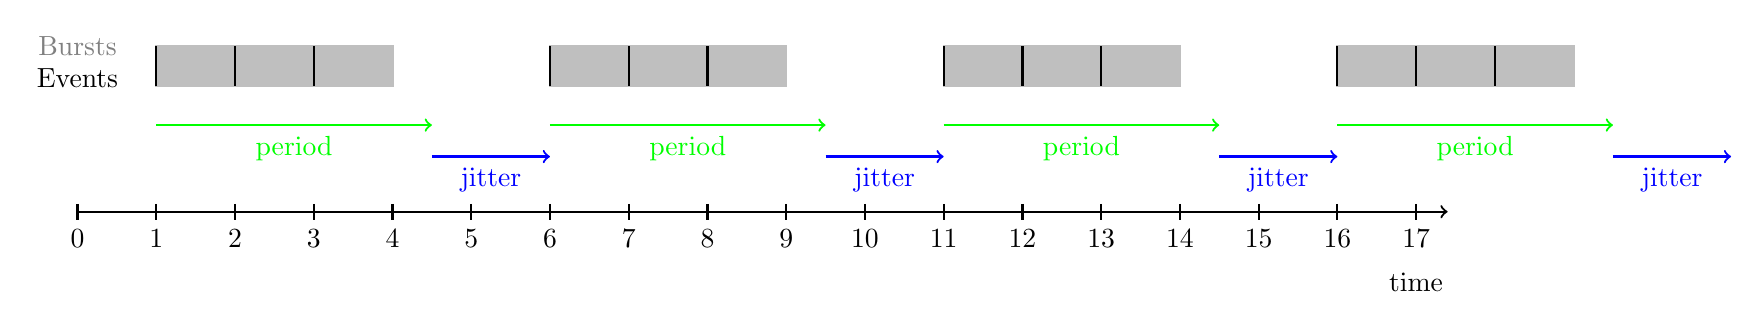
\begin{tikzpicture}[thick]
	% time axis
	\foreach \x in {0,...,17}
	\draw (\x,-4) -- (\x,-4.2) node[anchor=north] {\x};
	\draw[->] (0, -4.1) -- (17.4, -4.1);
	\node at(17, -5) {time};
	
	% bursts
	\node[gray] at (0, -2){Bursts};
	\draw [fill=lightgray, lightgray] (1, -2) rectangle (4,-2.5);
	\draw [fill=lightgray, lightgray] (6, -2) rectangle (9,-2.5);
	\draw [fill=lightgray, lightgray] (11, -2) rectangle (14,-2.5);
	\draw [fill=lightgray, lightgray] (16, -2) rectangle (19,-2.5);
	% events
	\node at (0, -2.4){Events};
	%\node at (0, -2.15){events};
	\foreach \x in {1, 6, 11, 16}
	{
		% events
		\draw[-] (\x, -2) -- (\x, -2.5);
		\draw[-] (\x+1, -2) -- (\x+1, -2.5);
		\draw[-] (\x+2, -2) -- (\x+2, -2.5);
		% periods
		\draw[->, green] (\x, -3) -- (\x+3.5, -3);
		\node[green] at (\x+1.75, -3.3){period};
		%jitters
		\draw[->, blue] (\x+3.5,-3.4) -- (\x+5, -3.4);
		\node[blue] at (\x+4.25, -3.7) {jitter};
	}
	\end{tikzpicture}
	\caption{BurstPatternEventTriggering Period-Jitter \textbf{accumulating}}
	\label{fig:BurstPatternEventTriggering1}
\end{figure}
\begin{figure}
	\centering
	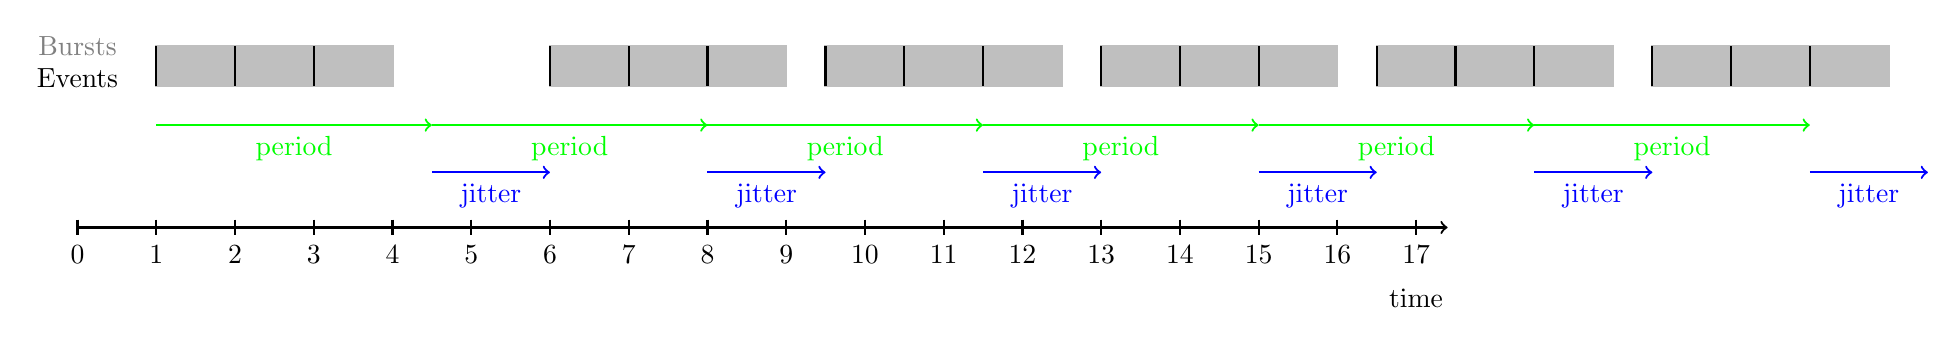
\begin{tikzpicture}[thick]
	% time axis
	\foreach \x in {0,...,17}
	\draw (\x,-4.2) -- (\x,-4.4) node[anchor=north] {\x};
	\draw[->] (0, -4.3) -- (17.4, -4.3);
	\node at(17, -5.2) {time};
	
	% bursts
	\node[gray] at (0, -2){Bursts};
	\draw [fill=lightgray, lightgray] (1, -2) rectangle (4,-2.5);
	\node at (0, -2.4){Events};
	
	%period 1
	\draw[->, green] (1, -3) -- (4.5, -3);
	\node[green] at (2.75, -3.3){period};
	
	% jitter 1
	\draw[->, blue] (4.5,-3.6) -- (6, -3.6);
	\node[blue] at (5.25, -3.9) {jitter};
	
	\foreach \y in {0, 1, 2}
	\draw[-] (1+\y, -2) -- (1+\y, -2.5);
	
	\foreach \x in {4.5, 8, 11.5, 15, 18.5}
	{
		% periods
		\draw[->, green] (\x, -3) -- (\x+3.5, -3);
		\node[green] at (\x+1.75, -3.3){period};
		% jitters
		\draw[->, blue] (\x+3.5,-3.6) -- (\x+5, -3.6);
		\node[blue] at (\x+4.25, -3.9) {jitter};
		%bursts	
		\draw [fill=lightgray, lightgray] (\x+1.5, -2) rectangle (\x+4.5,-2.5);
		% events
		\foreach \y in {0, 1, 2}
		\draw[-] (\x+\y+1.5, -2) -- (\x+\y+1.5, -2.5);
	}
	\end{tikzpicture}
	\caption{BurstPatternEventTriggering Period-Jitter \textbf{non-accumulating}}
	\label{fig:BurstPatternEventTriggering2}
\end{figure}

The combination of $patternPeriod$ and $patternJitter$ can be interpreted in an accumulating as seen in \ref{fig:BurstPatternEventTriggering1} or non-accumulating way as seen in \ref{fig:BurstPatternEventTriggering2} way. In the accumulating interpretation, the reference for the periodic occurrences is only the start point of the previous 

With the definition of $patternLength$ (\glqq time distance between the beginnings of subsequent repetitions of the given burst pattern\grqq) you would think, that the accumulating variant is meant. Against that, the period attribute in $PeriodicEventTriggering$-Constraint is also defined as \glqq distance between subsequent occurrences of the event\grqq in the text, hence it is understandable the accumulating way, but there is also the formal definition

\begin{math}
\exists t_{reference}\forall t_n: t_{reference}+(n+1)*period\leq t_n\leq t_{reference}+(n-1)*period+jitter,
\end{math}

where $t_n$ is the time of the $n$-th Event and $t_{reference}$ is a reference point, from which the periodic pattern starts, so the $PeriodicEventTriggering$-Constraint is meant to be understood in the non-accumulating way. It remains unclear, in which way the $BurstPatternEventTriggering$ is meant to be understood.

Another problem of the AUTOSAR Timing Extensions is, that they were made for design purposes, monitoring them can be difficult, as they may need continuously growing time and memory resources, which makes online monitoring impossible (more on monitorability in \ref{chapter-monitorability}). As example, we will use the burst pattern again, this time using the attributes as
\begin{itemize}
	\item
	$maxNumberOfOccurrences = INT\_MAX$
	\item
	$minNumberOfOccurrences = 1$
	\item
	$minimumInterArrivalTime = 0$
	\item
	$patternLength = 3$
	\item
	\textcolor{gray}{$patternPeriod$} \textcolor{gray}{unused}
	\item
	\textcolor{gray}{$patternJitter$} \textcolor{gray}{unused}
\end{itemize}

In \ref{fig:BurstPatternEventTriggering3} you see the application of the BurstPatternEventTriggering Constraint with the given parameters on a stream with events at the timestamps 3, 3.5, 4, 4.5. You can see the development of possible the burst cluster with ongoing time. The gray lines show, where the burst can lay, the black lines show, where they definitely are. In timestamp 3 with only one event so far, only one burst has to be considered and it can lay between timestamp 0 and 6, the only limitation is, that it must include timestamp 3 with the event in that point. In Timestamp 3.5, there are two events (at 3 and 3.5) so far and there are two possibilities for burst placements. The first possibility with only one burst with both events in it, and the second possibility, where the events are in different bursts. The third graphic shows the trace in timestamp 4 with three different events so far (3, 3.5, 4) and there are three different possibilities for burst placements to consider. One possible burst contains all three events, the second possibility has one burst with the event at timestamp 3 and one burst with the events at 3.5 and 4 and the third possibility has one Burst with the events at 3 and 3.5 and one burst with the event at 4. The possible bursts in graphic 4 are analog to the third graphic, one possibility with one burst containing all 4 events and 3 possibilities with the first burst containing the first event, the first and second event or the first, the second and the third event and the second burst containing the remaining events.\\
In this Example, we see, that it is possible to create an unlimited number of possibilities for burst placements within one burst length, when the \textit{minimumInterArrivalTime}-attribute is 0, which results in an infeasible resource consumption, as unlimited memory and time is needed to check the constraint in following events. Therefore, online monitoring this constraint is impossible in general, because of the strict resource limitations. More on that in \ref{chapter-monitorability}.

\begin{figure}
	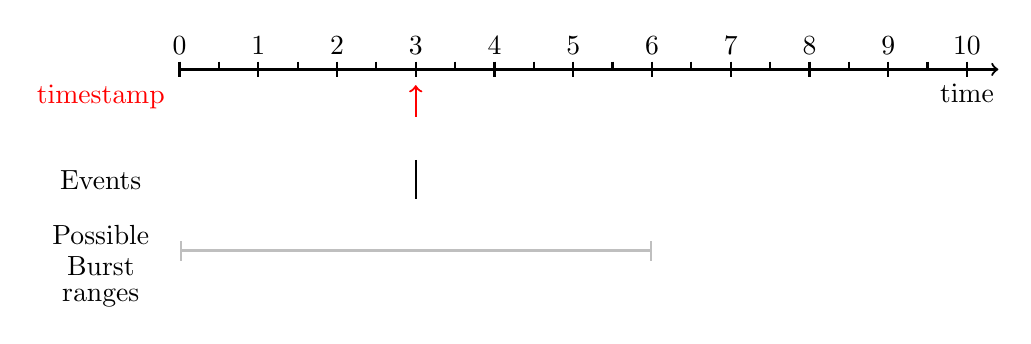
\begin{tikzpicture}[thick]
	%time axis
	\foreach \x in {0,...,10}
	{
		\draw (\x,0) -- (\x,-0.2);
		\node at (0+\x, 0.2) {\x};
	}
	\foreach \x in {0,...,9}
	\draw (\x+0.5,0) -- (\x+0.5,-0.1);
	\draw[->] (0, -0.1) -- (10.4, -0.1);
	\node at(10, -0.4) {time};
	
	\node[red] at(-1, -0.45) {timestamp};
	%watched time
	\draw[->, red] (3, -0.7)--(3, -0.3);
	
	\node at (-1, -1.5) {Events};
	\draw[-] (3, -1.25) -- (3, -1.75);
	
	\node at (-1, -2.2) {Possible};
	\node at (-1, -2.6) {Burst};
	\node at (-1, -3) {ranges};
	
	%Burst range
	\draw[|-|, lightgray] (0, -2.4) -- (6, -2.4);
	\end{tikzpicture}
	
	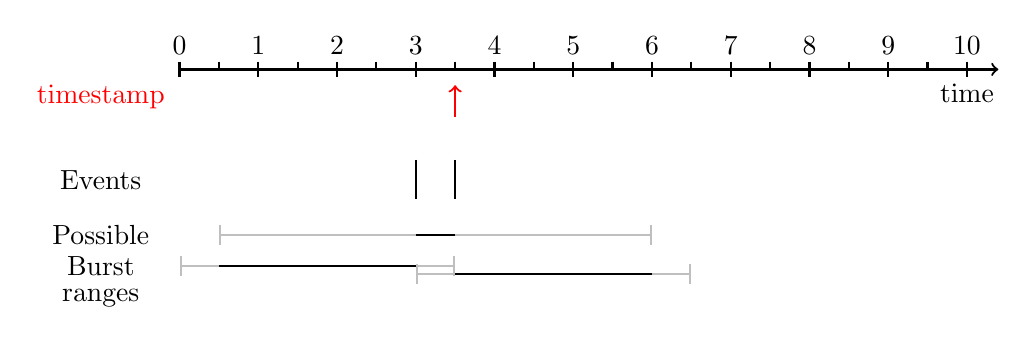
\begin{tikzpicture}[thick]
	%time axis
	\foreach \x in {0,...,10}
	{
		\draw (\x,0) -- (\x,-0.2);
		\node at (0+\x, 0.2) {\x};
	}
	\foreach \x in {0,...,9}
	\draw (\x+0.5,0) -- (\x+0.5,-0.1);
	\draw[->] (0, -0.1) -- (10.4, -0.1);
	\node at(10, -0.4) {time};
	
	\node[red] at(-1, -0.45) {timestamp};
	%watched time
	\draw[->, red] (3.5, -0.7)--(3.5, -0.3);
	
	\node at (-1, -1.5) {Events};
	\draw[-] (3, -1.25) -- (3, -1.75);
	\draw[-] (3.5, -1.25) -- (3.5, -1.75);
	
	\node at (-1, -2.2) {Possible};
	\node at (-1, -2.6) {Burst};
	\node at (-1, -3) {ranges};
	
	%Burst range 1
	\draw[|-|, lightgray] (0.5, -2.2) -- (6, -2.2);
	\draw[-] (3, -2.2) -- (3.5, -2.2);
	% Burst range 2
	\draw[|-|, lightgray] (0, -2.6) -- (3.5, -2.6);
	\draw[-] (0.5, -2.6) -- (3, -2.6);
	\draw[|-|, lightgray] (3, -2.7) -- (6.5, -2.7);
	\draw[-] (3.5, -2.7) -- (6, -2.7);
	\end{tikzpicture}
	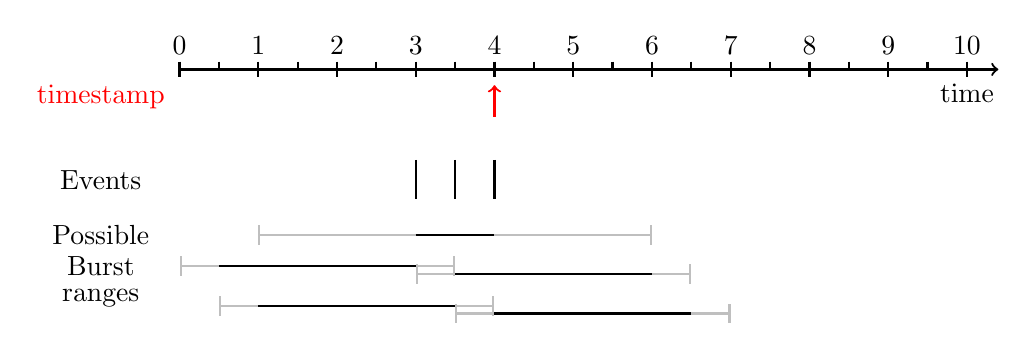
\begin{tikzpicture}[thick]
	%time axis
	\foreach \x in {0,...,10}
	{
		\draw (\x,0) -- (\x,-0.2);
		\node at (0+\x, 0.2) {\x};
	}
	\foreach \x in {0,...,9}
	\draw (\x+0.5,0) -- (\x+0.5,-0.1);
	\draw[->] (0, -0.1) -- (10.4, -0.1);
	\node at(10, -0.4) {time};
	
	\node[red] at(-1, -0.45) {timestamp};
	%watched time
	\draw[->, red] (4, -0.7)--(4, -0.3);
	
	\node at (-1, -1.5) {Events};
	\draw[-] (3, -1.25) -- (3, -1.75);
	\draw[-] (3.5, -1.25) -- (3.5, -1.75);
	\draw[-] (4, -1.25) -- (4, -1.75);
	
	\node at (-1, -2.2) {Possible};
	\node at (-1, -2.6) {Burst};
	\node at (-1, -3) {ranges};
	
	%Burst ranges poss. 1
	\draw[|-|, lightgray] (1, -2.2) -- (6, -2.2);
	\draw[-] (3, -2.2) -- (4, -2.2);
	% Burst ranges poss. 3 2.6,2.7
	\draw[|-|, lightgray] (0, -2.6) -- (3.5, -2.6);
	\draw[-] (0.5, -2.6) -- (3, -2.6);
	\draw[|-|, lightgray] (3, -2.7) -- (6.5, -2.7);
	\draw[-] (3.5, -2.7) -- (6, -2.7);
	% Burst ranges poss. 2
	\draw[|-|, lightgray] (0.5, -3.1) -- (4, -3.1);
	\draw[-] (1, -3.1) -- (3.5, -3.1);
	\draw[|-|, lightgray] (3.5, -3.2) -- (7, -3.2);
	\draw[-] (4, -3.2) -- (6.5, -3.2);
	\end{tikzpicture}
	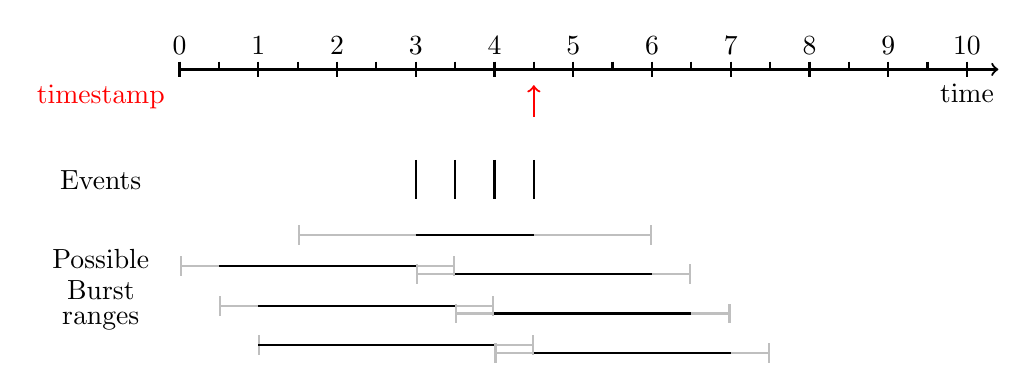
\begin{tikzpicture}[thick]
	%time axis
	\foreach \x in {0,...,10}
	{
		\draw (\x,0) -- (\x,-0.2);
		\node at (0+\x, 0.2) {\x};
	}
	\foreach \x in {0,...,9}
	\draw (\x+0.5,0) -- (\x+0.5,-0.1);
	\draw[->] (0, -0.1) -- (10.4, -0.1);
	\node at(10, -0.4) {time};
	
	\node[red] at(-1, -0.45) {timestamp};
	%watched time
	\draw[->, red] (4.5, -0.7)--(4.5, -0.3);
	
	\node at (-1, -1.5) {Events};
	\draw[-] (3, -1.25) -- (3, -1.75);
	\draw[-] (3.5, -1.25) -- (3.5, -1.75);
	\draw[-] (4, -1.25) -- (4, -1.75);
	\draw[-] (4.5, -1.25) -- (4.5, -1.75);
	
	\node at (-1, -2.5) {Possible};
	\node at (-1, -2.9) {Burst};
	\node at (-1, -3.3) {ranges};
	
	%Burst ranges poss. 1
	\draw[|-|, lightgray] (1.5, -2.2) -- (6, -2.2);
	\draw[-] (3, -2.2) -- (4.5, -2.2);
	% Burst ranges poss. 2
	\draw[|-|, lightgray] (0, -2.6) -- (3.5, -2.6);
	\draw[-] (0.5, -2.6) -- (3, -2.6);
	\draw[|-|, lightgray] (3, -2.7) -- (6.5, -2.7);
	\draw[-] (3.5, -2.7) -- (6, -2.7);
	% Burst ranges poss. 3
	\draw[|-|, lightgray] (0.5, -3.1) -- (4, -3.1);
	\draw[-] (1, -3.1) -- (3.5, -3.1);
	\draw[|-|, lightgray] (3.5, -3.2) -- (7, -3.2);
	\draw[-] (4, -3.2) -- (6.5, -3.2);
	% Burst ranges poss. 4
	\draw[|-|, lightgray] (1, -3.6) -- (4.5, -3.6);
	\draw[-] (1, -3.6) -- (4, -3.6);
	\draw[|-|, lightgray] (4, -3.7) -- (7.5, -3.7);
	\draw[-] (4.5, -3.7) -- (7, -3.7);
	\end{tikzpicture}
	\caption{BurstPatternEventTriggering Possible bursts, \textcolor{red}{$\uparrow$} shows the current time}
	\label{fig:BurstPatternEventTriggering3}
\end{figure}
\newpage

\section{TADL2}
	Because of the problems in the definitions and monitorability of the AUTOSAR Timing Extensions, the implementation of a monitor will be done on the TADL2 (Timing Augmented Description Language Version 2) Timing Constraints, which were defined in the TIMMO-2-USE project, which was developed as part of the EAST-ADL (Electronics Architecture and Software Technology-Architecture Description Language). EAST-ADL has similar goals as AUTOSAR, but the definitions are written in a more formalized fashion. The definitions of the AUTOSAR Timing Extensions are only textually described often, the TADL2-Definitions are defined in a more formal way, as they offer an formalized definition of each constraint in a timing constraint logic \cite{TIMMO2USE}. EAST-ADL is much less used in the automotive industry, but the EAST-ADL Timing Constraints are partly compatible to the AUTOSAR Timing Extensions, as they define sub- or subersets of each other. Many of the AUTOSAR Timing Extensions can be defined via a combination of TADL2 Constraints, as you will see in \ref{comparisonConstraints}.
	
\subsection{Parenthesis - Simple and Flexible Timing Constraint Logic}
	The formal definition of the TADL2 timing constraint are written in \emph{Timing Constraint Logic} (short: \emph{TiCL}), which was developed as part of the TIMMO-2-USE project. TiCL was formally introduced in \cite{TiCL}, for better understanding the key aspects of this article will be explained in the following.\\
	The main goal of TiCL is to be formal and expandable and offering the possibility of defining finite and infinite behaviors of events. In TiCL, only points in time, when events occur, are considered, therefore an events only consists of a real value as timestamp, without the possibility of adding a data value. There are 7 syntactic categories in TiCL
	\begin{align*}
		\mathbb{R} &\text{(arithmetic constants)}\\
		Avar &\text{(arithmetic variables)}\\
		AExp &\text{(arithmetic expressions)}\\[10pt]
		%\vspace{1cm}
		Svar &\text{(set variables)}\\
		SExp &\text{(set expressions)}\\[10pt]
		%\vspace{1cm}
		TVar &\text{(time variables)}\\
		CExp &\text{(constraint expressions)}
	\end{align*}
	Arithmetic expressions can be defined as arithmetic constants, arithmetic variables, application of $+,-,*,/$ on arithmetic expressions, application of the Cardinality operator on a set ($|E|$, $E\in SExp$) or as measure $\lambda(E)$ ($E\in SExp$). $\lambda(E)$ is defined as Lebesue measure, which is figuratively speaking, the length of all continuous intervals of $E$. In \ref{fig:TiCLMeasureExample} you see a visualized example of the measure operator $\lambda$. The set $E$ contains all Events between the timestamps $1$ and $9$, the set $F$ contains the events at the timestamps between 2 and 4 and 6 and 7, therefore $E\setminus F$ contains the events at the timestamps $\{1, 1.5, 4.5, 5, 5.5, 7.5, 8, 8.5, 9\}$.
	$E$ consists of one continuous interval from timestamp 1 to 9 with the length of 8, $F$ consists of two continuous intervals from 2 to 4 with the length of 2 and from 6 to 7 with the length of 1, therefore $\lambda(F)=3$. $E\setminus F$ consists of three continuous intervals, the first from 1 to 1.5 (length = 0.5), the second from 4.5 to 5.5 (length = 1) and the last from 7.5 to 9 (length = 1.5), so the total length of the continuous intervals of $E\setminus F$ is 3.\\
	% TODO richtig? vgl. executionTimeConstraint
	\begin{figure}
		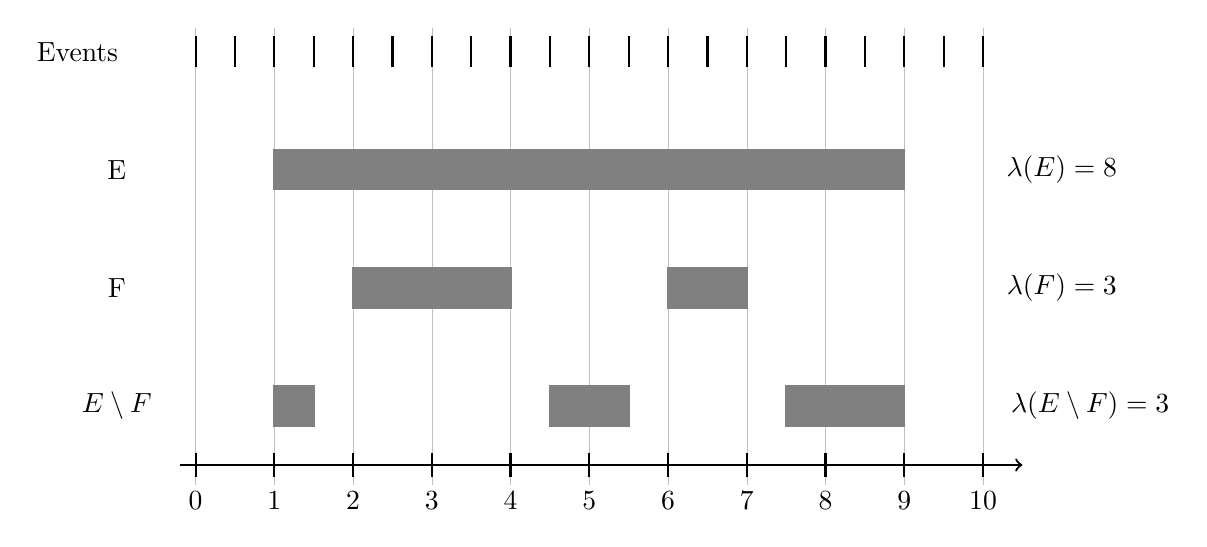
\begin{tikzpicture}[thick]
			\foreach \x in {0,...,10}
			{
				\draw[very thin, lightgray](\x, 1.8) -- (\x, -4);
				
				\draw (\x,-3.6) -- (\x,-3.9);
				\node at (0+\x, -4.2) {\x};
			}
			\draw[->] (-0.2, -3.75) -- (10.5, -3.75);
			
			\node at (-1,  0) {E};
			\draw [fill=gray,gray] (1,0.25) rectangle (9,-0.25); 
			
			\node at (-1, -1.5) {F};
			\draw [fill=gray,gray] (2,-1.25) rectangle (4,-1.75); 
			\draw [fill=gray,gray] (6,-1.25) rectangle (7,-1.75);
			
			\node at (-1, -3) {$E \setminus F$};
			\draw [fill=gray,gray] (1,-2.75) rectangle (1.5,-3.25); 
			\draw [fill=gray,gray] (4.5,-2.75) rectangle (5.5,-3.25);
			\draw [fill=gray,gray] (7.5,-2.75) rectangle (9,-3.25);
			
			\node at (11, 0) {$\lambda(E) = 8$};
			\node at (11, -1.5) {$\lambda(F) = 3$};
			\node at (11.36, -3) {$\lambda(E\setminus F) = 3$};
			
			\node at (-1.5, 1.5){Events};
			\foreach \x in {0, 0.5, ...,10}
			\draw (\x, 1.7) -- (\x, 1.3);
		\end{tikzpicture}
		\caption{Graphical example of $\lambda(E), \lambda(F)$ and $\lambda(E\setminus F)$}
		\label{fig:TiCLMeasureExample}
	\end{figure}	
	Set expressions can be defined as set variables, or as set of time variables fulfill a given constraint expression.\\
	Constraint expressions can be defined as application of the $\leq$-operator on time or arithmetic expressions, the $\in$ operator on time variables and set expressions, the logical conjunction on constraint expressions, the negation of constraint expressions and the $\forall$-Quantifier on arithmetic, set and time variables over an constraint expression.\\
	As extension to this definition, well known syntactic abbreviations like $true\equiv 0\leq 1$ or the $\exists$-quantifier will be used, but there are also some TiCL-specific syntactic abbreviations, which will be defined and explained in the following.\\
	\subsubsection{Interval Constructors}
		Let $x, y\in Tvar$ and $E, F\in SExp$.\\
		The constructor $[x\leq]$($[x<]$) is defined as ${y: x \leq y}$(${y: x < y}$), therefore the interval contains all points in time laying behind of $x$, possibly containing $x$.\\
		$[\leq x]$($[< x]$) is defined as complement of $[x<]$($[x\leq]$) and contains all timestamps laying before $x$.\\
		$[x..y]$ is defined as $[x\leq]\cap[<y]$, so all points of time after $x$, including $x$, and before $y$ are part of this interval.\\
		$[E \leq]$ is defined as $\{y : \exists x \in E : x \leq y\}$, this interval contains all point of time at and after the first timestamp in $E$. $[E<]$ is equal to $\{y : forall x \in E : x < y\}$, therefore it defines the interval containing all timestamps after the latest point of time in $E$.\\
		$[\leq E]$ ($[< E]$) is defined as $[E<]^C$ ($[E\leq]^C$), analogous to the operators on time variables.\\
		$[E]$ is equal to $[E\leq]\cap[\leq E]$. It defines the time interval between the first and last element of $E$, including these points in time.\\
		$E_{x<}$($E_{<x}$) is defined as $E\cap [x<]$($E\cap [<x]$). This operators filters the timestamps in $E$ so that only the points in time before (after) remain.\\
		$[x..E]$ equals $[x\leq]\cap[<(E_{x<})]$. The interval begins at $x$ and ends right before the first element of $E$ after $x$.\\
		$[E..F]$ is defined as $\{x:\exists y\in E:x\in[y..F]\}$ and describes the intervals, where the previous operator is applied on every element of $E$.\\
	% TODO ? es gibt noch mehr, nur einfügen, wenn benötigt.
	% TODO x-y/y-x
	% TODO Index in Eventmenge -> hier oder in nächster subsection (in TADL neu definiert)
	% TODO X\leq Y -> X is subsequence of Y
\subsection{TADL2-Timing Constraints}
	For better understanding of the following chapters, the TADL Constraints will be presented next. As abbreviation and unification, all timing expressions are defined as set $\mathbb{T}$, which are understood as real numbers but expanded with $\infty$ and $-\infty$ in this chapter, but other value ranges for time expressions are possible and will be used in other parts of this thesis.\\
	We define an event as a time value combined with an data value. The range of the data values are arbitrary, infinite data types are possible, also as empty data types, when only the point in time is relevant for the event. All TADL constraints are defined with attributes, which can be sets of events and timing or arithmetic expressions.
	\subsubsection{DelayConstraint}
		The \emph{DelayConstraint} has 4 attributes
		\begin{align*}
			\emph{source} & \hspace{.5cm}\text{event set}\\
			\emph{target} & \hspace{.5cm}\text{event set}\\
			\emph{lower}  & \hspace{.5cm}\text{$\mathbb{T}$ (time expression)}\\
			\emph{upper}  & \hspace{.5cm}\text{$\mathbb{T}$}
		\end{align*}
		and is defined as\\[10pt]
		\begin{math}
			\forall x\in source:\exists y\in target: lower\leq y-x\leq upper.
		\end{math}\\[10pt]
		For all events $x$ in \emph{source}, there must be an $y$ event in \emph{target}, so that $y$ lays between \emph{lower} and \emph{upper} 'after' $x$. Note, that \emph{lower} and \emph{upper} can have negative values and that additional events in \emph{target}, without an associated \emph{source} are allowed.\\
		In \ref{fig:delayConstraintExample} you see a visualized example of the \emph{DelayConstraint} with the attributes $lower=2$, $upper=3$, $source=\{1, 5, 6\}$ and $target=\{2, 3.5, 5, 7, 8.2, 9\}$. The first element of source at timestamp 1 results in a required event in target between the timestamp 3 and 4 that is fulfilled by the event at 3.5. The second event of source requires an target event between 7 and 8, fulfilled by the event at 7. The last event of source is satisfied by the target event at 8.2 and 9.
		\begin{figure}
			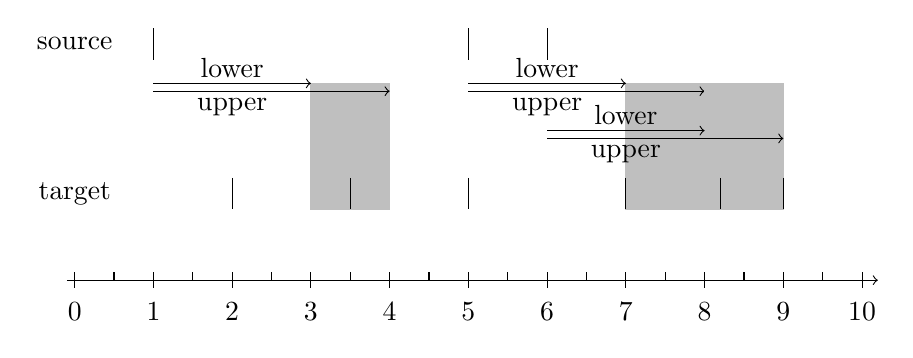
\begin{tikzpicture}
				% source events
				\node[] at (0,-0.2){source};
				\draw (1, 0) -- (1, -0.4);
				\draw (5, 0) -- (5, -0.4);
				\draw (6, 0) -- (6, -0.4);
				
				% upper/lower 1
				\draw [fill=lightgray, lightgray] (3, -0.7) rectangle (4,-2.3);
				\node at (2, -0.5){lower};
				\node at (2, -1){upper};
				\draw[->] (1,-0.7) -- (3, -0.7);
				\draw[->] (1, -0.8) -- (4, -0.8);
				
				
				% upper/lower 2
				\draw [fill=lightgray, lightgray] (7, -0.7) rectangle (8,-2.3);
				\node at (6, -0.5){lower};
				\node at (6, -1){upper};
				\draw[->] (5,-0.7) -- (7, -0.7);
				\draw[->] (5, -0.8) -- (8, -0.8);
				
				% upper/lower 3
				\draw [fill=lightgray, lightgray] (8, -0.7) rectangle (9,-2.3);
				\node at (7, -1.1){lower};
				\node at (7, -1.6){upper};
				\draw[->] (6,-1.3) -- (8, -1.3);
				\draw[->] (6, -1.4) -- (9, -1.4);
				% target events
				\node[] at (0,-2.1){target};
				\draw (2, -1.9) -- (2, -2.3);
				\draw (3.5, -1.9) -- (3.5, -2.3);
				\draw (5, -1.9) -- (5, -2.3);
				\draw (7, -1.9) -- (7, -2.3);
				\draw (8.2, -1.9) -- (8.2, -2.3);
				\draw (9, -1.9) -- (9, -2.3);
				
				\foreach \x in {0, 1, ..., 10}{
					\draw (\x, -3.1) -- (\x, -3.3);
					\node at(\x, -3.6) {\x};
				}
			
				\foreach \x in {0.5, 1.5, ..., 9.5}
					\draw (\x, -3.1) -- (\x, -3.2);
				\draw[->] (-0.1, -3.2) -- (10.2, -3.2);
					
			\end{tikzpicture}
			\caption{Example DelayConstraint - $lower = 2$, $upper = 3$}
			\label{fig:delayConstraintExample}
		\end{figure}
	\subsubsection{StrongDelayConstraint}
		The \emph{StrongDelayConstraint} has 4 attributes
		\begin{align*}
			\emph{source} & \hspace{.5cm}\text{event set}\\
			\emph{target} & \hspace{.5cm}\text{event set}\\
			\emph{lower}  & \hspace{.5cm}\text{$\mathbb{T}$ (time expression)}\\
			\emph{upper}  & \hspace{.5cm}\text{$\mathbb{T}$}
		\end{align*}
		and is defined as\\[10pt]
		\begin{math}
			|source| = |target| \land\\
			\forall i: \forall x: x=source(i) \Rightarrow \exists y: y=target(i)\land lower\leq y-x\leq upper.
		\end{math}\\[10pt]
		The \emph{StrongDelayConstraint} is a stricter version of the \emph{DelayConstraint}, as it requires a bijective assignment between the source and target events, therefore additional events in target without matching source event are not allowed. In \ref{fig:StrongDelayConstraintExample} you see an example of the \emph{StrongDelayConstraint}. The example is the same as in the previous constraint, but without the additional target events at 2, 5 and 8.2.
 		\begin{figure}
		 	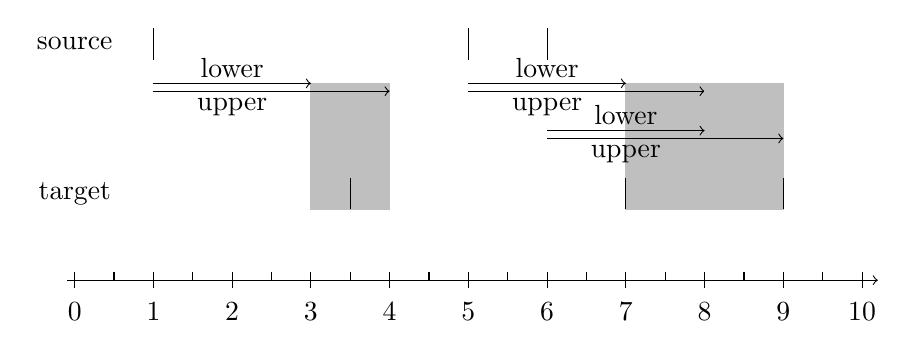
\begin{tikzpicture}
		 	% source events
		 	\node[] at (0,-0.2){source};
		 	\draw (1, 0) -- (1, -0.4);
		 	\draw (5, 0) -- (5, -0.4);
		 	\draw (6, 0) -- (6, -0.4);
		 	
		 	% upper/lower 1
		 	\draw [fill=lightgray, lightgray] (3, -0.7) rectangle (4,-2.3);
		 	\node at (2, -0.5){lower};
		 	\node at (2, -1){upper};
		 	\draw[->] (1,-0.7) -- (3, -0.7);
		 	\draw[->] (1, -0.8) -- (4, -0.8);
		 	
		 	
		 	% upper/lower 2
		 	\draw [fill=lightgray, lightgray] (7, -0.7) rectangle (8,-2.3);
		 	\node at (6, -0.5){lower};
		 	\node at (6, -1){upper};
		 	\draw[->] (5,-0.7) -- (7, -0.7);
		 	\draw[->] (5, -0.8) -- (8, -0.8);
		 	
		 	% upper/lower 3
		 	\draw [fill=lightgray, lightgray] (8, -0.7) rectangle (9,-2.3);
		 	\node at (7, -1.1){lower};
		 	\node at (7, -1.6){upper};
		 	\draw[->] (6,-1.3) -- (8, -1.3);
		 	\draw[->] (6, -1.4) -- (9, -1.4);
		 	% target events
		 	\node[] at (0,-2.1){target};
		 	\draw (3.5, -1.9) -- (3.5, -2.3);
		 	\draw (7, -1.9) -- (7, -2.3);
		 	\draw (9, -1.9) -- (9, -2.3);
		 	
		 	\foreach \x in {0, 1, ..., 10}{
		 		\draw (\x, -3.1) -- (\x, -3.3);
		 		\node at(\x, -3.6) {\x};
		 	}
		 	
		 	\foreach \x in {0.5, 1.5, ..., 9.5}
		 	\draw (\x, -3.1) -- (\x, -3.2);
		 	\draw[->] (-0.1, -3.2) -- (10.2, -3.2);
		 	
		 	\end{tikzpicture}
		 	\caption{Example StrongDelayConstraint - $lower = 2$, $upper = 3$}
		 	\label{fig:StrongDelayConstraintExample}
		 \end{figure}
	\subsubsection{RepeatConstraint}
		The \emph{RepeatConstraint} also has 4 attributes
		\begin{align*}
			\emph{event} & \hspace{.5cm}\text{event set}\\
			\emph{lower} & \hspace{.5cm}\text{$\mathbb{T}$ (time expression)}\\
			\emph{upper} & \hspace{.5cm}\text{$\mathbb{T}$}\\
			\emph{span}	 & \hspace{.5cm}\text{$int$}\\
		\end{align*}
		and is defined as\\[10pt]
		\begin{math}
			\forall X\leq event: |X|=span+1\Rightarrow lower \leq \lambda([X])\leq upper.
		\end{math}\\[10pt]
		As reminder, the $A\leq B$-operator over two sets of events $A, B$ describes, that $A$ is a sub-sequence of $B$, the $\lambda(A)$-function calculates the total length of all continuous intervals in $A$ and the $[A]$ returns the time interval between the oldest and newest event in $A$.
		The definition specifies that the length of each time interval containing $span+1$ consecutively events must be between $upper$ and $lower$.\\
		The idea behind this constraint is to define repeated occurrences of events, with the possibility of overlapping, specified by the \emph{span} attribute. After any event $x$, there are $span-1$ events and than the next event must be between $lower$ and $upper$ after $x$.\\
		In \ref{fig:RepeatConstraintExample1} you see an example of the RepeatConstraint with the attributes $event=\{1,3,5,...\}$, $lower=upper=2$ and $span=1$. Because $lower$ is equal $upper$ and $span$ is 1, the events are following a strict periodic pattern after the first event. \ref{fig:RepeatConstraintExample2} shows a more complex example with events at $\{0, 2, 4, 7, 9, 11,...\}$, $lower=4$, $upper=5$ and $span=2$. The $span$-attribute is 2, so the time distance between all subsequent events with an even index are considered, just like the subsequent events with an uneven index. 
		
		\begin{figure}
			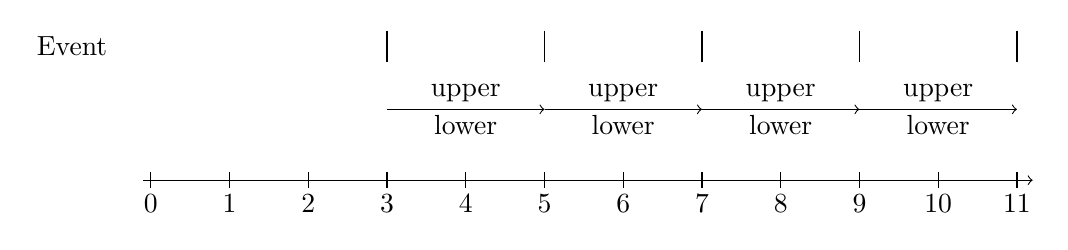
\begin{tikzpicture}
				% events
				\node at(-1 , 0.2){Event}; 
				\foreach \x in {3,5,...,9}{
					\draw (\x, 0.4) -- (\x, 0);
					\draw[->] (\x, -0.6) -- (\x+2, -0.6);
					\node at(\x+1, -0.8){lower};
					\node at(\x+1, -0.4){upper};
				}
				\draw (11, 0.4) -- (11, 0);
				% time axis
				\foreach \x in {0,...,11}{
					\draw (\x, -1.4) -- (\x, -1.6);
					\node at(\x, -1.8){\x};
				}
				\draw[->] (-0.1, -1.5) -- (11.2, -1.5);
			\end{tikzpicture}
			\caption{Example RepeatConstraint - $lower = 2$, $upper = 2$, $span = 1$}
			\label{fig:RepeatConstraintExample1}
		\end{figure}
	
		\begin{figure}
			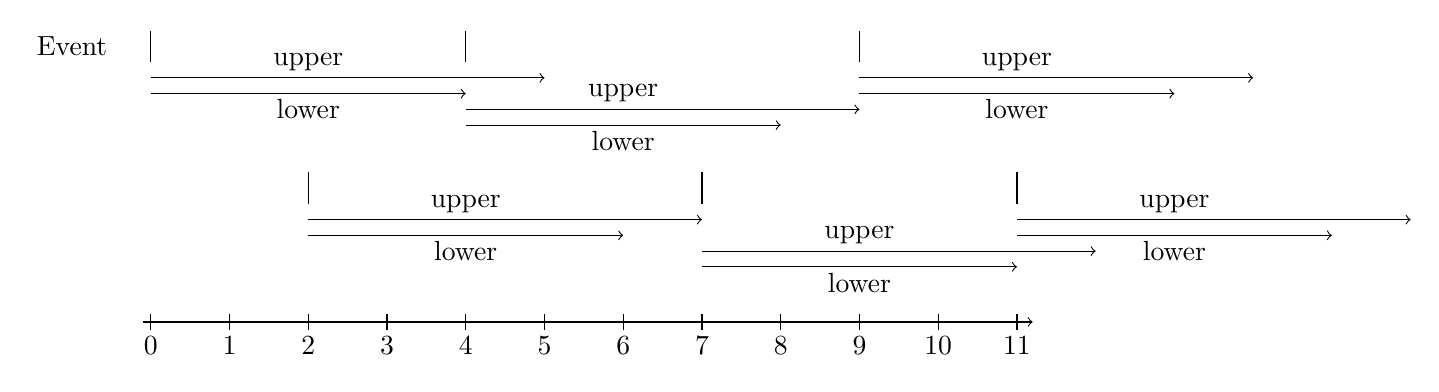
\begin{tikzpicture}
				\node at(-1, 0.2){Event};
				%eventreihe 1
				\foreach \x in {0, 4, 9} {
					\draw (\x,0) -- (\x, 0.4);
				}
				\foreach \x in {0, 9} {
					\node at (\x+2, 0) {upper};
					\draw[->] (\x, -0.2) -- (\x+5, -0.2);
					\draw[->] (\x, -0.4) -- (\x+4, -0.4);
					\node at (\x+2, -0.6) {lower};
				}
				\foreach \x in {4} {
					\node at (\x+2, -0.4) {upper};
					\draw[->] (\x, -0.6) -- (\x+5, -0.6);
					\draw[->] (\x, -0.8) -- (\x+4, -0.8);
					\node at (\x+2, -1) {lower};
				}
				%eventreihe 2
				\foreach \x in {2, 7, 11} {
					\draw (\x,-1.4) -- (\x, -1.8);
				}
				\foreach \x in {2, 11} {
					\node at (\x+2, -1.8) {upper};
					\draw[->] (\x, -2) -- (\x+5, -2);
					\draw[->] (\x, -2.2) -- (\x+4, -2.2);
					\node at (\x+2, -2.4) {lower};
				}
				\foreach \x in {7} {
					\node at (\x+2, -2.2) {upper};
					\draw[->] (\x, -2.4) -- (\x+5, -2.4);
					\draw[->] (\x, -2.6) -- (\x+4, -2.6);
					\node at (\x+2, -2.8) {lower};
				}
				%time axis
				\foreach \y in {-3.2}{
					\foreach \x in {0,...,11}{
						\draw (\x, \y) -- (\x, \y-0.2);
						\node at(\x, \y-0.4){\x};
					}
					\draw[->] (-0.1, \y-0.1) -- (11.2, \y-0.1);
				}
			\end{tikzpicture}
			\caption{Example RepeatConstraint - $lower = 4$, $upper = 5$, $span = 2$}
			\label{fig:RepeatConstraintExample2}
		\end{figure}
	
	\subsubsection{RepetitionConstraint}
		The \emph{RepetitionConstraint} has 5 attributes
		\begin{align*}
			\emph{event} & \hspace{.5cm}\text{event set}\\
			\emph{lower} & \hspace{.5cm}\text{$\mathbb{T}$ (time expression)}\\
			\emph{upper} & \hspace{.5cm}\text{$\mathbb{T}$}\\
			\emph{span}	 & \hspace{.5cm}\text{$int$}\\
			\emph{jitter}& \hspace{.5cm}\mathbb{T}
		\end{align*}
		and is defined via the \emph{RepeatConstraint} and the \emph{StrongDelayConstraint} as\\[10pt]
		\begin{math}
			\exists X: RepeatConstraint(X, lower, upper, span) \land \\
			\text{\hspace{1cm}}StrongDelayConstraint(X, event, 0, jitter)
		\end{math}\\[10pt]
		where $X$ is a set of arbitrary time stamps, that follow the structure of the \emph{RepeatConstraint}(various(\emph{span}) loose periodic repetitions). The actual points in time of \emph{event} lay between the timestamps of $X$ and $jitter$ after that. For each point of time there is one, and only one, corresponding timestamp in $X$.
		In \ref{fig:RepetitionConstraintExample} you see an example of the \emph{RepetitionConstraint} with the attributes $event=\{0.5, 3.3, 4.7, 7.6, 9.9, ...\}$, $lower=4$, $upper=5$, $span=2$ and $jitter=1$. The shown timestamps of $X$ are only one possibility and may change due to later elements of $event$.
		
		\begin{figure}			
			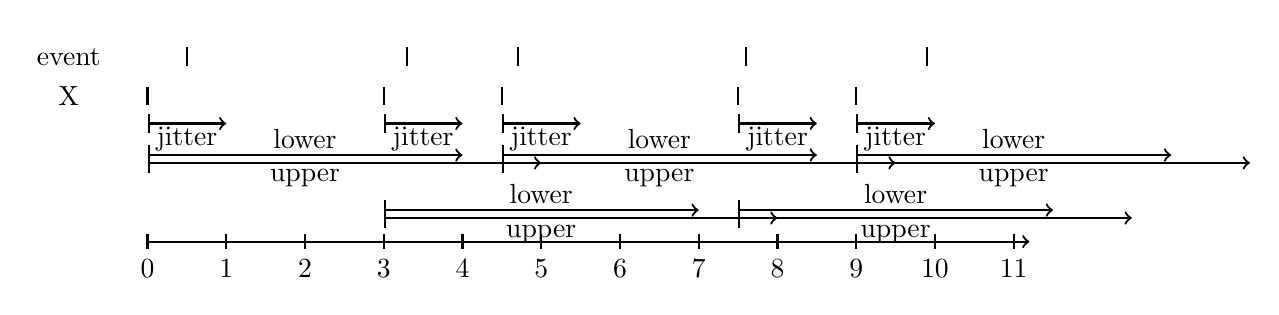
\begin{tikzpicture}[thick]
				% time axis
				\foreach \x in {0,...,11}
				\draw (\x,-2) -- (\x,-2.2)
					node[anchor=north] {\x};
				\draw[->] (0, -2.1) -- (11.2, -2.1);
				
				%Event 1
				\node[] at (0.5,0) (event1){};
				\node[] at (0.5,0.5) (event1_below){};
				\draw[] (event1) -- (event1_below);
				
				% X 1
				\node[] at (0,0) (x1){};
				\node[] at (0,-0.5) (x1_below){};
				\draw[] (x1) -- (x1_below);
				%jitter 1
				\node at (0.5,-0.8) (){jitter};
				\draw[|->] (0,-0.6) -- (1,-0.6);
				%lower 1
				\node at (2,-0.8) (){lower};
				\draw[|->] (0,-1) -- (4,-1);
				%lower 1
				\node at (2,-1.3) (){upper};
				\draw[|->] (0,-1.1) -- (5,-1.1);
				
				%Event 2
				\node[] at (4.7,0) (event2){};
				\node[] at (4.7,0.5) (event2_below){};
				\draw[] (event2) -- (event2_below);
				% X 2
				\node[] at (4.5,0) (x2){};
				\node[] at (4.5,-0.5) (x2_below){};
				\draw[] (x2) -- (x2_below);
				%jitter 2
				\node at (5,-0.8) (){jitter};
				\draw[|->] (4.5,-0.6) -- (5.5,-0.6);
				%lower 2
				\node at (6.5,-0.8) (){lower};
				\draw[|->] (4.5,-1) -- (8.5,-1);
				%lower 2
				\node at (6.5,-1.3) (){upper};
				\draw[|->] (4.5,-1.1) -- (9.5,-1.1);
				
				%Event 1
				\node[] at (9.9,0) (event1){};
				\node[] at (9.9,0.5) (event1_below){};
				\draw[] (event1) -- (event1_below);
				% X 3
				\node[] at (9,0) (x3){};
				\node[] at (9,-0.5) (x3_below){};
				\draw[] (x3) -- (x3_below);
				%jitter 3
				\node at (9.5,-0.8) (){jitter};
				\draw[|->] (9,-0.6) -- (10,-0.6);
				%lower 3
				\node at (11,-0.8) (){lower};
				\draw[|->] (9,-1) -- (13,-1);
				%lower 3
				\node at (11,-1.3) (){upper};
				\draw[|->] (9,-1.1) -- (14,-1.1);
				
				%Event 1
				\node[] at (3.3,0) (event1){};
				\node[] at (3.3,0.5) (event1_below){};
				\draw[] (event1) -- (event1_below);
				% X 4
				\node[] at (3,0) (x4){};
				\node[] at (3,-0.5) (x4_below){};
				\draw[] (x4) -- (x4_below);
				%jitter 4
				\node at (3.5,-0.8) (){jitter};
				\draw[|->] (3,-0.6) -- (4,-0.6);
				%lower 4
				\node at (5,-1.5) (){lower};
				\draw[|->] (3,-1.7) -- (7,-1.7);
				%lower 4
				\node at (5,-2) (){upper};
				\draw[|->] (3,-1.8) -- (8,-1.8);
				
				%Event 1
				\node[] at (7.6,0) (event1){};
				\node[] at (7.6,0.5) (event1_below){};
				\draw[] (event1) -- (event1_below);
				% X 5
				\node[] at (7.5,0) (x5){};
				\node[] at (7.5,-0.5) (x5_below){};
				\draw[] (x5) -- (x5_below);
				%jitter 4
				\node at (8,-0.8) (){jitter};
				\draw[|->] (7.5,-0.6) -- (8.5,-0.6);
				%lower 4
				\node at (9.5,-1.5) (){lower};
				\draw[|->] (7.5,-1.7) -- (11.5,-1.7);
				%lower 4
				\node at (9.5,-2) (){upper};
				\draw[|->] (7.5,-1.8) -- (12.5,-1.8);
				
				\node at(-1, 0.25){event};
				\node at(-1, -0.25){X};
			\end{tikzpicture}
			\caption{Example RepetitionConstraint - $lower = 4$, $upper = 5$, $span = 2$, $jitter=1$}
			\label{fig:RepetitionConstraintExample}
		\end{figure}
		
	
	\subsubsection{SynchronizationConstraint}
		The \emph{SynchronizationConstraint} has 2 attributes
		\begin{align*}
			\emph{event} & \hspace{.5cm}\text{set of event sets, $|event|\geq 2$}\\
			\emph{tolerance} & \hspace{.5cm}\mathbb{T}
		\end{align*}
		and is defined via the \emph{DelayConstraint} as\\[10pt]
		\begin{math}
			\exists X: \forall i: DelayConstraint(X, event_i, 0, tolerance) \land\\
			\text{\hspace{1cm}}DelayConstraint(event_i, X, -tolerance, 0)
		\end{math}\\[10pt]
		$X$ is a set of arbitrary point in time an there must be at least one timestamp in each set of \emph{event}, that is between an element of $X$ and $tolerance$ after that. Also, for each element in any set of \emph{event}, there must be a matching element of $X$.\\
		In \ref{fig:SynchronizationConstraintExample} is an example of the \emph{SynchronizationConstraint} with the attributes $event=\{\{0.5, 3, 7, 7.5\}, \{0.7, 2.5, 7.3, 7.8\}, \{1.2, 3.2, 3.3, 3.4, 7.6, 8.4\}\}$ and $tolerance = 1$. The first points in time of each element of event form the first cluster, the corresponding element of $X$ can be between $0.2$ and $0.5$. For simplification, only the latest possible value for the element of $X$ are shown. In the second cluster of events you see that multiple timestamps from one element of $event$ can be associated with a single element of $X$. The third and fourth cluster show, that overlapping is also possible.
		\begin{figure}			
			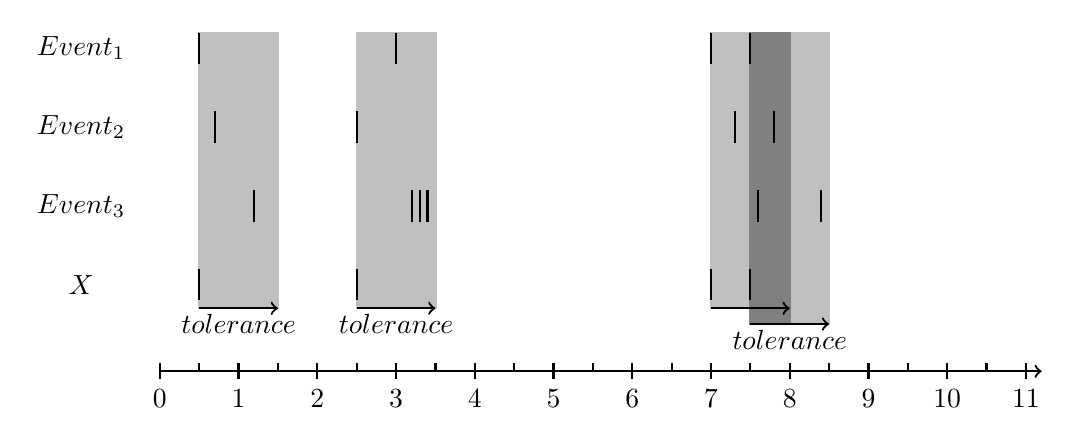
\begin{tikzpicture}[thick]
				% tolerance rectangles
				\foreach \x in {0.5, 2.5, 7}
					\draw [fill=lightgray, lightgray] (\x, 0.2) rectangle (\x+1, -3.3);
				\draw [fill=lightgray, lightgray] (7.5, 0.2) rectangle (8.5, -3.5);
				\draw [fill=gray, gray] (7.5, 0.2) rectangle (8, -3.5);
				% time axis
				\foreach \y in {-4}{
					\foreach \x in {0,...,11}
						\draw (\x,\y) -- (\x,\y-0.2) node[anchor=north] {\x};
					\foreach \x in {0.5,1.5,...,10.5}
						\draw (\x,\y) -- (\x,\y-0.1);
					\draw[->] (0,\y-0.1) -- (11.2, \y-0.1);
				}
				
				\node at (-1, 0){$Event_1$};
				\foreach \x in {0.5, 3, 7, 7.5}
					\draw (\x, 0.2) -- (\x, -0.2);
				
				\node at (-1, -1){$Event_2$};
				\foreach \x in {0.7, 2.5, 7.3, 7.8}
					\draw (\x, -0.8) -- (\x, -1.2);
				
				\node at (-1, -2){$Event_3$};
				\foreach \x in {1.2, 3.2, 3.3, 3.4, 7.6, 8.4}
					\draw (\x, -1.8) -- (\x, -2.2);
					
				\node at (-1, -3){$X$};
				\foreach \x in {0.5, 2.5}{
					\draw (\x, -2.8) -- (\x, -3.2);
					\draw[->] (\x, -3.3) -- (\x+1, -3.3);
					\node at (\x+0.5, -3.5){$tolerance$};
				}
				\foreach \x in {7}{
					\draw (\x, -2.8) -- (\x, -3.2);
					\draw[->] (\x, -3.3) -- (\x+1, -3.3);
				}
				\foreach \x in {7.5}{
					\draw (\x, -2.8) -- (\x, -3.2);
					\draw[->] (\x, -3.5) -- (\x+1, -3.5);
					\node at (\x+0.5, -3.7){$tolerance$};
				}
					
			\end{tikzpicture}
			\caption{Example SynchronizationConstraint - $tolerance = 1$}
			\label{fig:SynchronizationConstraintExample}
		\end{figure}
		
		
		
	\subsubsection{StrongSynchronizationConstraint}
		The \emph{StrongSynchronizationConstraint} has the same two attributes as the \emph{SynchronizationConstraint}
		\begin{align*}
			\emph{event} & \hspace{.5cm}\text{set of event sets, $|event|\geq 2$}\\
			\emph{tolerance} & \hspace{.5cm}\mathbb{T}
		\end{align*}
		and is defined as\\[10pt]
		\begin{math}
			\exists X: \forall i: StrongDelayConstraint(X, event_i, 0, tolerance)
		\end{math}\\[10pt]
		The \emph{StrongSynchronizationConstraint} is a stricter variant of the \emph{SynchronizationConstraint}, as it requires a bijective assignment between the elements of $X$ to one element of each set of $event$. For every $x\in X$, only one corresponding timestamp per set in $event$ is allowed, like you can see in \ref{fig:StrongSynchronizationConstraintExample}, which shows the same example as the one for the \emph{SynchronizationConstraint}, but the excess time stamps at $3.2$ and $3.3$ have been removed.
			\begin{figure}			
				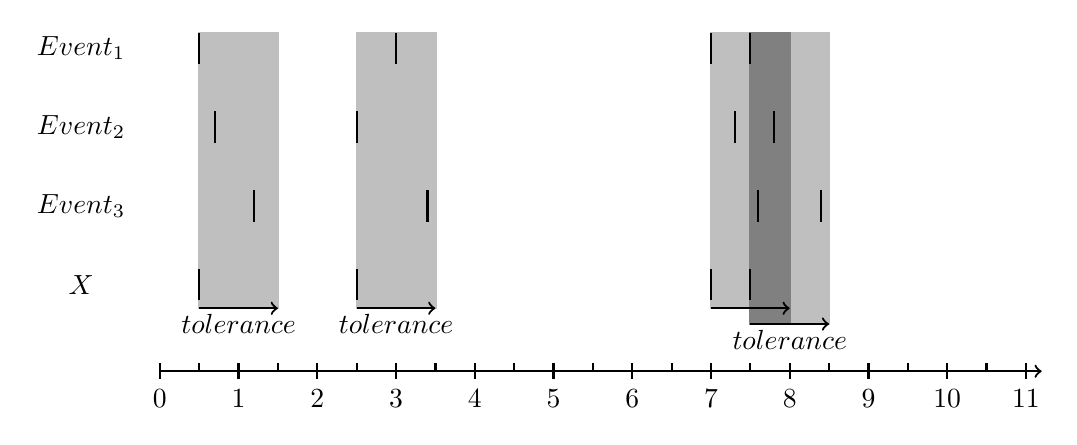
\begin{tikzpicture}[thick]
				% tolerance rectangles
				\foreach \x in {0.5, 2.5, 7}
				\draw [fill=lightgray, lightgray] (\x, 0.2) rectangle (\x+1, -3.3);
				\draw [fill=lightgray, lightgray] (7.5, 0.2) rectangle (8.5, -3.5);
				\draw [fill=gray, gray] (7.5, 0.2) rectangle (8, -3.5);
				% time axis
				\foreach \y in {-4}{
					\foreach \x in {0,...,11}
					\draw (\x,\y) -- (\x,\y-0.2) node[anchor=north] {\x};
					\foreach \x in {0.5,1.5,...,10.5}
					\draw (\x,\y) -- (\x,\y-0.1);
					\draw[->] (0,\y-0.1) -- (11.2, \y-0.1);
				}
				
				\node at (-1, 0){$Event_1$};
				\foreach \x in {0.5, 3, 7, 7.5}
				\draw (\x, 0.2) -- (\x, -0.2);
				
				\node at (-1, -1){$Event_2$};
				\foreach \x in {0.7, 2.5, 7.3, 7.8}
				\draw (\x, -0.8) -- (\x, -1.2);
				
				\node at (-1, -2){$Event_3$};
				\foreach \x in {1.2, 3.4, 7.6, 8.4}
				\draw (\x, -1.8) -- (\x, -2.2);
				
				\node at (-1, -3){$X$};
				\foreach \x in {0.5, 2.5}{
					\draw (\x, -2.8) -- (\x, -3.2);
					\draw[->] (\x, -3.3) -- (\x+1, -3.3);
					\node at (\x+0.5, -3.5){$tolerance$};
				}
				\foreach \x in {7}{
					\draw (\x, -2.8) -- (\x, -3.2);
					\draw[->] (\x, -3.3) -- (\x+1, -3.3);
				}
				\foreach \x in {7.5}{
					\draw (\x, -2.8) -- (\x, -3.2);
					\draw[->] (\x, -3.5) -- (\x+1, -3.5);
					\node at (\x+0.5, -3.7){$tolerance$};
				}
			
			\end{tikzpicture}
			\caption{Example StrongSynchronizationConstraint - $tolerance = 1$}
			\label{fig:StrongSynchronizationConstraintExample}
		\end{figure}
		
		
	\subsubsection{ExecutionTimeConstraint}
		The \emph{ExecutionTimeConstraints} takes 4 attributes
		\begin{align*}
			\emph{start} & \hspace{.5cm}\text{set of events}\\
			\emph{stop} & \hspace{.5cm}\text{set of events}\\
			\emph{preempt} & \hspace{.5cm}\text{set of events}\\
			\emph{resume} & \hspace{.5cm}\text{set of events}\\
			\emph{lower} & \hspace{.5cm}\mathbb{T}\\
			\emph{upper} & \hspace{.5cm}\mathbb{T}\\
		\end{align*}
		and is defined as\\[10pt]
		\begin{math}
			\forall x\in start: lower\leq \lambda([x..stop]\setminus[preempt..resume]) \leq upper
		\end{math}\\[10pt]
		The interval constructor $\forall x\in start: [x..stop]$ defines the time interval between each point in time of $start$ until the next element of $stop$, excluding the $stop$ timestamp. $[preempt..resume]$, which is removed from the considered interval length, defines the intervals between each element of preempt until the next timestamp of resume.\\
		The Idea behind this constraint is to test the run time of a task, without counting interruptions.
		\ref{fig:ExecutionTimeConstraintExample} shows an example of the \emph{ExecutionTimeConstraints} with $start=\{1\}$, $end=\{7\}$, $preempt=\{2, 5\}$ and $resume = \{3, 6.5\}$. Therefore, $[start..end]$ spans the interval from time 1 to 7 with the length of 6 and $[preempt..resume]$ spans two intervals, 2 to 3 and 5 to 6.5 with the length 1 and 1.5. As result, $\lambda([x..stop]\setminus[preempt..resume])$ for $x = 1$ is 3.5 and the constraint is fulfilled, if, and only if, lower is equal or \emph{lower} than 3.5 and \emph{upper} is greater than that.\\
		\begin{figure}
   			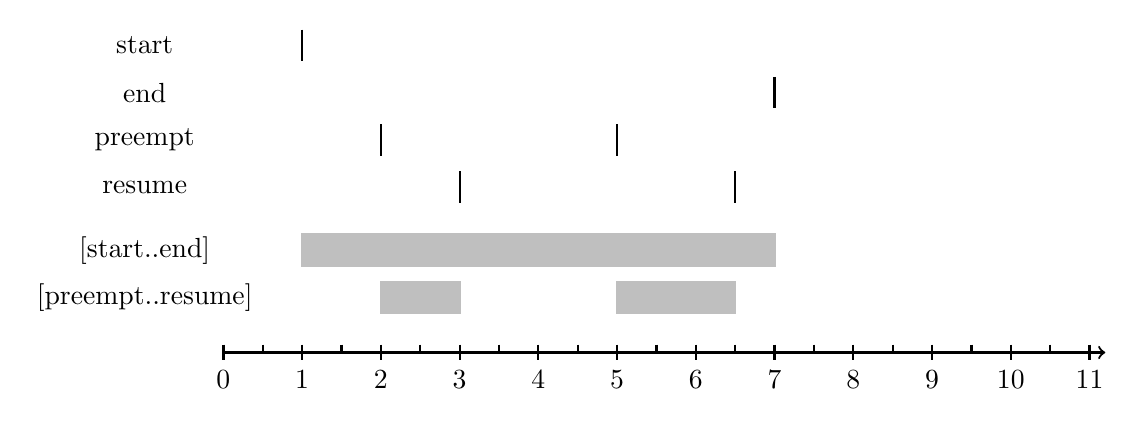
\begin{tikzpicture}[thick]
				% time axis
				\foreach \y in {-4}{
					\foreach \x in {0,...,11}
					\draw (\x,\y) -- (\x,\y-0.2) node[anchor=north] {\x};
					\foreach \x in {0.5,1.5,...,10.5}
					\draw (\x,\y) -- (\x,\y-0.1);
					\draw[->] (0,\y-0.1) -- (11.2, \y-0.1);
				}
				% start
				\node at (-1, -0.2) {start};
				\draw[] (1,0) -- (1,-0.4);
				% end
				\node at (-1, -0.8) {end};
				\draw[] (7, -0.6) -- (7, -1);
				%preempt
				\node at (-1, -1.4) {preempt};
				\draw[] (2, -1.2) -- (2, -1.6);
				\draw[] (5, -1.2) -- (5, -1.6);
				%resume
				\node at (-1, -2) {resume};
				\draw[] (3, -1.8) -- (3, -2.2);
				\draw[] (6.5, -1.8) -- (6.5, -2.2);
				
				\node at (-1, -2.8) {[start..end]};
				\draw [fill=lightgray, lightgray] (1, -2.6) rectangle (7, -3.0);
				
				\node at (-1, -3.4) {[preempt..resume]};
				\draw [fill=lightgray, lightgray] (2, -3.2) rectangle (3, -3.6);
				\draw [fill=lightgray, lightgray] (5, -3.2) rectangle (6.5, -3.6);
			\end{tikzpicture}
			\caption{Example ExecutionTimeConstraint}
			\label{fig:ExecutionTimeConstraintExample}
		\end{figure}
		
	\subsubsection{OrderConstraint}
		The \emph{OrderConstraint} takes two attributes
		\begin{align*}
			\emph{source} & \hspace{.5cm}\text{set of events}\\
			\emph{target} & \hspace{.5cm}\text{set of events}
		\end{align*}
		and is defined as\\[10pt]
		\begin{math}
			|source| = |target| \land \forall i:\exists x: x=source(i)\Rightarrow \exists y: y=target(i)\land < x \leq y
		\end{math}\\[10pt]
		This constraints ensures the order of events, so that the $i$-th event of $target$ is after the $i$-th event of $source$. Also, the number of events in \emph{source} and \emph{target} must be equal.\\
		In \ref{fig:OrderConstraintExample} you see an example of the \emph{OrderConstraint} with $source = \{1, 4, 6, 7\}$ and $target = \{3, 5, 9, 9.5\}$. The constraint is fulfilled, because the number of elements is equal for both sets and each $i$-th timestamp in \emph{target} is later that the $i$-th timestamp of $source$.
		\begin{figure}
			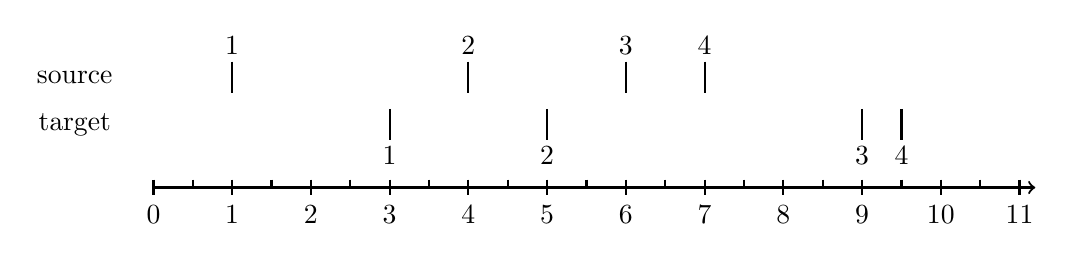
\begin{tikzpicture}[thick]
				% time axis
				\foreach \y in {-1.5}{
					\foreach \x in {0,...,11}
					\draw (\x,\y) -- (\x,\y-0.2) node[anchor=north] {\x};
					\foreach \x in {0.5,1.5,...,10.5}
					\draw (\x,\y) -- (\x,\y-0.1);
					\draw[->] (0,\y-0.1) -- (11.2, \y-0.1);
				}
				% start
				\node at (-1, -0.2) {source};
				\foreach \x in {1, 4, 6, 7}{
					\draw[] (\x,0) -- (\x,-0.4);
				}
				\node at (1, 0.2) {1};
				\node at (4, 0.2) {2};
				\node at (6, 0.2) {3};
				\node at (7, 0.2) {4};
				% end
				\node at (-1, -0.8) {target};
				\foreach \x in {3, 5, 9, 9.5}{
					\draw[] (\x,-0.6) -- (\x,-1);
				}
				\node at (3, -1.2) {1};
				\node at (5, -1.2) {2};
				\node at (9, -1.2) {3};
				\node at (9.5, -1.2) {4};
			\end{tikzpicture}
			\caption{Example OrderConstraint}
			\label{fig:OrderConstraintExample}
		\end{figure}
		
		
	\subsubsection{ComparisonConstraint}
		The \emph{ComparisonConstraint} is significant different to all previous and following constraints, as it does not describe the behavior of events, and only compares two timing expressions. It takes 3 attributes
		\begin{align*}
			\emph{leftOperand} 	& \hspace{.5cm}\mathbb{T}\\
			\emph{rightOperand} & \hspace{.5cm}\mathbb{T}\\
			\emph{operator}		& \hspace{.5cm} \text{comparisonOperator}(\in \{LessThanOrEqual, LessThan,\\
								& \hspace{3.5cm} GreaterThanOrEqual, GreaterThan, Equal\})
		\end{align*}
		The definition is pretty straight forward as it only applies the given operator to the operands:\\[10pt]
		\begin{math}
			ComparisonConstraint(leftOperand, rightOperand, LessThanOrEqual)\\
				\Leftrightarrow leftOperand \leq rightOperand\\[5pt]
			ComparisonConstraint(leftOperand, rightOperand, LessThan)\\
				\Leftrightarrow leftOperand < rightOperand\\[5pt]
			ComparisonConstraint(leftOperand, rightOperand, GreaterThanOrEqual)\\
				\Leftrightarrow leftOperand \geq rightOperand\\[5pt]
			ComparisonConstraint(leftOperand, rightOperand, GreaterThan)\\
				\Leftrightarrow leftOperand > rightOperand\\[5pt]
			ComparisonConstraint(leftOperand, rightOperand, Equal)\\
				\Leftrightarrow leftOperand = rightOperand
		\end{math}\\[10pt]
		Due to the simplicity of this constraint, no explicit example is given.
		
	\subsubsection{SporadicConstraint}
		The \emph{SporadicConstraint} takes 5 attributes
		\begin{align*}
			\emph{event} 	& \hspace{.5cm}\text{set of events}\\
			\emph{lower} 	& \hspace{.5cm}\mathbb{T}\\
			\emph{upper} 	& \hspace{.5cm}\mathbb{T}\\
			\emph{jitter}	& \hspace{.5cm}\mathbb{T}\\
			\emph{minimum}	& \hspace{.5cm}\mathbb{T}\\
		\end{align*}
		and is defined via the \emph{Repetition}- and the \emph{RepeatConstraint} as\\[10pt]
		\begin{math}
			RepetitionConstraint(event, lower, upper, 1, jitter)\\
			\land RepeatConstraint(event, minimum, \infty, 1)
		\end{math}\\[10pt]
		The second part of the definition, using the \emph{RepeatConstraint}, ensures that all events in \emph{event} lay at least \emph{minimum} apart. The application of the \emph{RepetitionConstraint} generates a set of events $X$, that lay between $lower$ and $upper$ apart. For each point of time in $X$, there must be exactly one timestamp in \emph{event}, that is not before the corresponding entry of $X$ and not later than \emph{jitter} after that.\\
		\ref{fig:SporadicConstraintExample} shows a possible utilization of the \emph{SporadicConstraint} with the attributes $lower=2$, $upper=2.5$, $jitter=1$, $minimum=2$ and $event=\{1, 3.5, 6, 8.2, 10.5,...\}$. As in the \emph{RepetitionConstraint}, the exact position of the timestamps in $X$ is variable and may need to be changed due to later entries in $event$.
		%TODO minimum in example
		\begin{figure}
			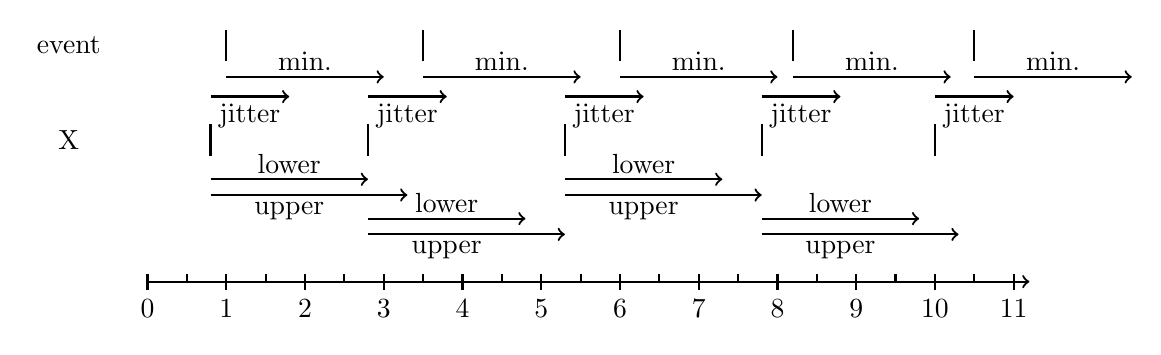
\begin{tikzpicture}[thick]
			% time axis
			\foreach \y in {-2.5}{
				\foreach \x in {0,...,11}
				\draw (\x,\y) -- (\x,\y-0.2) node[anchor=north] {\x};
				\foreach \x in {0.5,1.5,...,10.5}
				\draw (\x,\y) -- (\x,\y-0.1);
				\draw[->] (0,\y-0.1) -- (11.2, \y-0.1);
			}
			% event
			\node at (-1, 0.4) {event};
			\foreach \x in {1, 3.5, 6, 8.2, 10.5}{
				\draw[] (\x,0.2) -- (\x,+0.6);
				%minimum
				\draw[->] (\x, 0) -- (\x+2, 0);
				\node at (\x+1, 0.2) {min.};
			}
			% X
			\node at (-1, -0.8) {X};
			\foreach \x in {0.8, 2.8, 5.3, 7.8, 10}{
				\draw[] (\x,-0.6) -- (\x,-1);
				%jitter
				\draw[->] (\x, -0.25) -- (\x+1, -0.25);
				\node at (\x+0.5, -0.5) {jitter};
			}
			%lower/upper
			\foreach \x in {0.8, 5.3}{
				\node at (\x+1, -1.1){lower};
				\draw[->] (\x, -1.3) -- (\x+2, -1.3);
				\draw[->] (\x, -1.5) -- (\x+2.5, -1.5);
				\node at (\x+1, -1.7){upper};
			}
			\foreach \x in {2.8, 7.8}{
				\node at (\x+1, -1.6){lower};
				\draw[->] (\x, -1.8) -- (\x+2, -1.8);
				\draw[->] (\x, -2) -- (\x+2.5, -2);
				\node at (\x+1, -2.2){upper};
			}

			\end{tikzpicture}
			\caption{Example SporadicConstraint - $lower=2$, $upper=2.5$, $jitter=1$, $minimum=2$}
			\label{fig:SporadicConstraintExample}
		\end{figure}
	
	\subsubsection{PeriodicConstraint}
		The \emph{PeriodicConstraint} takes 4 attribute
		\begin{align*}
			\emph{event} 	& \hspace{.5cm}\text{set of events}\\
			\emph{period} 	& \hspace{.5cm}\mathbb{T}\\
			\emph{jitter}	& \hspace{.5cm}\mathbb{T}\\
			\emph{minimum}	& \hspace{.5cm}\mathbb{T}\\
		\end{align*}
		and defines a specialized form of the \emph{SporadicConstraint}\\[10pt]
		\begin{math}
			SporadicConstraint(event, period, period, jitter, minimum)
		\end{math}\\[10pt]
		The variable timestamps in the set $X$ are now following a strictly periodic pattern, where subsequent elements of this set lay exactly \emph{period} apart. Each element of \emph{event} lays between one element of $X$ and \emph{jitter} after that. Again, there must be bijective mapping between the elements of \emph{event} and $X$.\\
		In \ref{fig:PeriodicConstraintExample}, the \emph{PeriodicConstraint} with the attributes $period=3$, $jitter=1$, $minimum=2.5$ and $event = \{1.2, 4.0, 8, 10.6, ...\}$ is visualized. The timestamps of $X$ lay exactly \emph{period} apart and the $events$ behind that in the previously described way. Also, the minimum time distance between all points of time in \emph{event} is minimum.
		\begin{figure}
			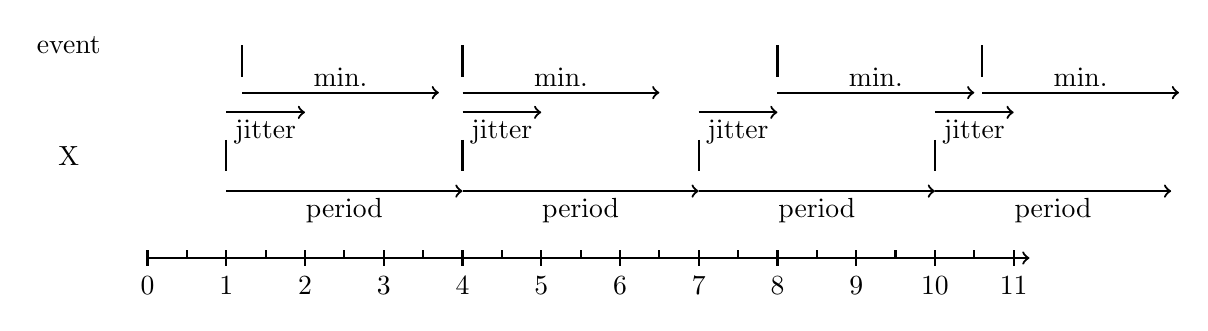
\begin{tikzpicture}[thick]
			% time axis
			\foreach \y in {-2}{
				\foreach \x in {0,...,11}
				\draw (\x,\y) -- (\x,\y-0.2) node[anchor=north] {\x};
				\foreach \x in {0.5,1.5,...,10.5}
				\draw (\x,\y) -- (\x,\y-0.1);
				\draw[->] (0,\y-0.1) -- (11.2, \y-0.1);
			}
			% event
			\node at (-1, 0.6) {event};
			\foreach \x in {1.2, 4.0, 8, 10.6}{
				%timestamp
				\draw[] (\x,0.2) -- (\x,+0.6);
				%minimum
				\draw[->] (\x, 0) -- (\x+2.5, 0);
				\node at (\x+1.25, 0.2) {min.};
			}
			% X
			\node at (-1, -0.8) {X};
			\foreach \x in {1, 4, 7, 10}{
				%timestamp
				\draw[] (\x,-0.6) -- (\x,-1);
				%jitter
				\draw[->] (\x, -0.25) -- (\x+1, -0.25);
				\node at (\x+0.5, -0.5) {jitter};
				%period
				\draw[->] (\x, -1.25) -- (\x+3, -1.25);
				\node at (\x+1.5, -1.5) {period};
			}
			\end{tikzpicture}
			\caption{Example SporadicConstraint - $period=3$, $jitter=1$, $minimum=2.5$}
			\label{fig:PeriodicConstraintExample}
		\end{figure}
		
		
	\subsubsection{PatternConstraint}
	\subsubsection{ArbitraryConstraint}
	\subsubsection{BurstConstraint}
	\subsubsection{ReactionConstraint}
	\subsubsection{AgeConstraint}
	\subsubsection{OutputSynchronizationConstraint}
	\subsubsection{InputSynchronizationConstraint}
			
\subsection{Comparison TADL2 - AUTOSAR Timing Extension}
\label{comparisonConstraints}
	

